\section{Kontekstuelle begrænsninger}

\begin{frame}
\frametitle{Kontekstuelle begrænsninger}
\begin{center}
\begin{itemize}
\item Hvad er kontekstuelle begrænsninger?
\item Hvilke begrænsninger har \productname{}?
\item ScopeChecker
\end{itemize}
\end{center}
\end{frame}

%***TYPER***

%DET KAN VI
\begin{frame}[fragile]
\frametitle{Typer}

\keyword{define} \constant{foo} = \type{A}[].\constant{bar} \\
\keyword{type} \type{A}[]\{ \\
  \quad  \keyword{define} \constant{bar} = \numeral{10} \\
\}

\begin{itemize}                                  
\item Anvendte typer kan bindes til én og kun én erklæring
\item Typer har de medlemmer, der tilgås
\end{itemize}
\end{frame}

\begin{frame}[fragile]
\input{billeder/tikz/typedef}



\end{frame}

\begin{frame}[fragile]
\frametitle{Typer}

\keyword{define} \constant{foo} = \type{A}[].\constant{bar}[\numeral{3},
\numeral{7}] \\
\keyword{type} \type{A}[]\{ \\
  \quad  \keyword{define} \constant{bar} = \numeral{10} \\
\}

\begin{itemize}                                  
\item \textcolor{red}{Tjekke korrespondance mellem formelle / aktuelle parametre}
\end{itemize}

\end{frame}

\begin{frame}[fragile]
\frametitle{Typer}
\keyword{define} \constant{foo} = \keyword{let} \variable{a} = \type{B}[] \\
\qquad \qquad \qquad \keyword{in} \variable{a}.\constant{bar} \\
\keyword{type} \type{A}[]\{ \\
  \quad \keyword{define} \constant{bar} = \numeral{10} \\
\} \\
\keyword{type} \type{B}[]\{\\

\}

\begin{itemize}                                  
\item \textcolor{red}{Inferere en variabels type}
\end{itemize}

\end{frame}

\begin{frame}[fragile]
\frametitle{Typer}

\keyword{define} \constant{someobject} = \type{A}[\numeral{1}, \numeral{2}]\\
\keyword{type} \type{A}[\variable{a}, \variable{b}]\\
\keyword{type} \type{B}[] \keyword{extends} \type{A}[\numeral{1}, \numeral{2}]\\

\begin{itemize}                                  
\item Instantiering foregår med korrekt antal parametre
\item Subtype kalder supertype med korrekt antal parametre
\item Supertype eksisterer!
\end{itemize}

\end{frame}

\begin{frame}[fragile]
\frametitle{Typer}
\keyword{type} \type{A}[] \keyword{extends} \type{B}[]\\
\keyword{type} \type{B}[] \keyword{extends} \type{C}[]\\
\keyword{type} \type{C}[] \keyword{extends} \type{A}[]\\

\begin{itemize}                                 
\item Ingen cyklisk nedarvning
\end{itemize}
\end{frame}

\begin{frame}[fragile]
\begin{figure}[ht]
  \begin{center}
    \begin{tikzpicture}[level/.style={sibling distance=30mm/#1}]      
      \node [square] (a) {$\mathbf{A}$};
      \node [square, yshift=-4em, xshift=-2.5em] (b) {$\mathbf{B}$};
      \node [square, yshift=-4em, xshift=2.5em] (d) {$\mathbf{D}$};
      \node [square, yshift=-8em, xshift=-5em] (c) {$\mathbf{C}$};
      \node [square, yshift=0em, xshift=12em] (e) {$\mathbf{E}$};
      \node [square, yshift=-4em, xshift=12em] (f) {$\mathbf{F}$};

      \draw[<-, thick,] (a) -- (b);
      \draw[<-, thick,] (b) -- (c);
      \draw[<-, thick,] (a) -- (d);
      \draw[<-, thick,] (e) -- (f);
    \end{tikzpicture}
  \end{center}
\end{figure}
\end{frame}

\begin{frame}[fragile]
\begin{figure}[ht]
  \begin{center}
    \begin{tikzpicture}[level/.style={sibling distance=30mm/#1}]      
      \node [square] (a) {$\mathbf{A_2}$};
      \node [square, yshift=-4em, xshift=-2.5em] (b) {$\mathbf{B_1}$};
      \node [square, yshift=-4em, xshift=2.5em] (d) {$\mathbf{D_0}$};
      \node [square, yshift=-8em, xshift=-5em] (c) {$\mathbf{C_0}$};
      \node [square, yshift=0em, xshift=12em] (e) {$\mathbf{E_1}$};
      \node [square, yshift=-4em, xshift=12em] (f) {$\mathbf{F_0}$};

      \draw[<-, thick,] (a) -- (b);
      \draw[<-, thick,] (b) -- (c);
      \draw[<-, thick,] (a) -- (d);
      \draw[<-, thick,] (e) -- (f);
    \end{tikzpicture}
  \end{center}
\end{figure}
\end{frame}

\begin{frame}[fragile]
\begin{figure}[ht]
  \begin{center}
    \begin{tikzpicture}[level/.style={sibling distance=30mm/#1}]      
      \node [square] (a) {$\mathbf{A_1}$};
      \node [square, yshift=-4em, xshift=-2.5em] (b) {$\mathbf{B_0}$};
      \node [square, yshift=0em, xshift=12em] (e) {$\mathbf{E_0}$};

      \draw[<-, thick,] (a) -- (b);
    \end{tikzpicture}
  \end{center}
\end{figure}
\begin{itemize}
 \item Topologisk sorteret sekvens: C, D, F
 \end{itemize}
\end{frame}

\begin{frame}[fragile]
\begin{figure}[ht]
  \begin{center}
    \begin{tikzpicture}[level/.style={sibling distance=30mm/#1}]      
      \node [square] (a) {$\mathbf{A_0}$};
    \end{tikzpicture}
  \end{center}
\end{figure}
\begin{itemize}
  \item Topologisk sorteret sekvens: C, D, F, B, E
  \end{itemize}
\end{frame}

\begin{frame}[fragile] 
  \begin{itemize}
    \item Topologisk sorteret sekvens: C, D, F, B, E, A
    \end{itemize}
 
 	\begin{figure}[ht]
  \begin{center}
    \begin{tikzpicture}[level/.style={sibling distance=30mm/#1}]      
      \node [square] (a) {$\mathbf{A_1}$};
      \node [square, yshift=-4em, xshift=-2.5em] (b) {$\mathbf{B_1}$};
      \node [square, yshift=-4em, xshift=+2.5em] (c) {$\mathbf{C_1}$};
      
      \draw[<-, thick,] (a) -- (b);
      \draw[<-, thick,] (b) -- (c);
      \draw[<-, thick,] (c) -- (a);
    \end{tikzpicture}
  \end{center}
\end{figure}

\begin{itemize}
  \item Omvendt: A, E, B, F, D, C
  \end{itemize}
\end{frame}


\begin{frame}[fragile] 
\begin{table}[h]
\begin{tabular}{|l|l|l|}
 \cline{1-1} \cline{3-3} 
Figur          &  & KantFigur : Figur    \\ \cline{1-1} \cline{3-3} 
\textcolor{gray}{areal} &  &                      \\
               &  &  \textcolor{gray}{antalKanter} \\
               &  &                      \\
               &  &                      \\ \cline{1-1} \cline{3-3} 
\end{tabular}
\end{table}
\begin{table}[h]
\begin{tabular}{|l|l|l|}
 \cline{1-1} \cline{3-3} 
 Firkant : KantFigur &  & AnvendtFirkant : Firkant    \\ \cline{1-1} \cline{3-3} 
areal      &  &                      \\
antalKanter     &  &                      \\
\textcolor{gray}{h}          &  & h               \\
\textcolor{gray}{b}          &  & b              \\ \cline{1-1} \cline{3-3} 
\end{tabular}
\end{table}
\end{frame}

\begin{frame}[fragile] 
\begin{table}[h]
\begin{tabular}{|l|l|l|}
 \cline{1-1} \cline{3-3} 
Figur          &  & KantFigur : Figur    \\ \cline{1-1} \cline{3-3} 
\textcolor{gray}{areal} &  & \textcolor{gray}{areal}       \\
               &  & \textcolor{gray}{antalKanter} \\
               &  &                      \\
               &  &                      \\ \cline{1-1} \cline{3-3} 
\end{tabular}
\end{table}
\begin{table}[h]
\begin{tabular}{|l|l|l|}
 \cline{1-1} \cline{3-3} 
Firkant : KantFigur &  & AnvendtFirkant : Firkant       \\ \cline{1-1} \cline{3-3} 
areal               &  &                      \\
antalKanter         &  &                      \\
\textcolor{gray}{h}          &  & h                    \\
\textcolor{gray}{b}          &  & b                    \\ \cline{1-1} \cline{3-3} 
\end{tabular}
\end{table} 	
\end{frame}

\begin{frame}[fragile] 
\begin{table}[h]
\begin{tabular}{|l|l|l|}
 \cline{1-1} \cline{3-3} 
Figur          &  & KantFigur : Figur    \\ \cline{1-1} \cline{3-3} 
\textcolor{gray}{areal} &  & \textcolor{gray}{areal}       \\
               &  & \textcolor{gray}{antalKanter} \\
               &  &                      \\
               &  &                      \\ \cline{1-1} \cline{3-3} 
\end{tabular}
\end{table}
\begin{table}[h]
\begin{tabular}{|l|l|l|}
 \cline{1-1} \cline{3-3} 
Firkant : KantFigur &  & AnvendtFirkant : Firkant       \\ \cline{1-1} \cline{3-3} 
areal               &  & areal                \\
antalKanter         &  & antalKanter          \\
\textcolor{gray}{h}          &  & h                    \\
\textcolor{gray}{b}          &  & b                    \\ \cline{1-1} \cline{3-3} 
\end{tabular}
\end{table}
\end{frame}

\begin{frame}[fragile] 
\begin{table}[h]
\begin{tabular}{|l|l|l|}
 \cline{1-1} \cline{3-3} 
Figur          &  & KantFigur : Figur    \\ \cline{1-1} \cline{3-3} 
\textcolor{gray}{areal} &  & \textcolor{gray}{areal}       \\
               &  & \textcolor{gray}{antalKanter} \\
               &  &                      \\
               &  &                      \\ \cline{1-1} \cline{3-3} 
\end{tabular}
\end{table}
\begin{table}[h]
\begin{tabular}{|l|l|l|}
 \cline{1-1} \cline{3-3} 
Firkant : KantFigur &  & AnvendtFirkant : Firkant       \\ \cline{1-1} \cline{3-3} 
areal               &  & areal                \\
antalKanter         &  & antalKanter          \\
\textcolor{gray}{h}          &  & h                    \\
\textcolor{gray}{b}          &  & b                    \\ \cline{1-1} \cline{3-3} 
\end{tabular}
\end{table}
\begin{center}
\texttt{AnvendtFirkant[].areal} $\rightarrow$ ok

\texttt{Firkant[].h} $\rightarrow$ \textcolor{red}{ikke tilladt}

Abstrakte typer identificeres
\end{center}
\end{frame}

%CONSTANTS
\begin{frame}[fragile]
\frametitle{Variabler}

\keyword{let} \variable{a} = \numeral{2}, \variable{b} = \numeral{3}\\ 
\quad \keyword{in} \ldots\\
\vspace{0.25cm}
\constant{add}[\variable{a}, \variable{b}] = \ldots\\
\vspace{0.25cm}
\texttt{\#}[\variable{a}, \variable{b}] \texttt{=>} \ldots\\
\vspace{0.25cm}
\keyword{type} \type{A}[]\{\\
\quad \keyword{data} \variable{a}\\
\quad \keyword{data} \variable{b}\\
\quad \ldots\\
\}

\begin{itemize}                                  
\item Åbner nyt scope
\item Variabler tilføjes til nuværende scope
\end{itemize}

\end{frame}

\begin{frame}[fragile]
\frametitle{Variabler}
\keyword{let} \variable{a} = \numeral{2}, \variable{b} = \numeral{3}
\keyword{in} \\
\quad  \keyword{let} \variable{a} = \numeral{5}, \variable{f} = \numeral{7}
\keyword{in}\\
\quad \quad \variable{a} + \variable{b} + \variable{f}

\begin{center}
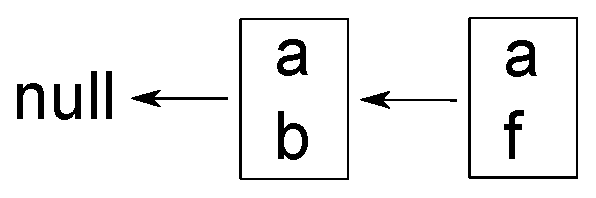
\includegraphics[height=1.5cm]{../report/pictures/scope2}
\end{center}
\begin{itemize}
  \item Variabel erklæres, som allerede findes i aktivt scope = \textcolor{red}{ScopeError}
\end{itemize}

\end{frame}

%VARIABLER



